%%%%%%%%%%%%%%%%%%%%%%%%%%%%%%%%%%%%%%%%%%%%%%%%%%%%%%%%%%%%
%%  This Beamer template was created to be a simple and clean.
%%  Anyone can freely use or modify it for any purpose without
%%  attribution.
%%
%%  The starting point for this template was [1] with further
%%  inspiration from [2].  Logo taken from [3].
%%
%%  [1] http://cameron.bracken.bz/beamer-template
%%  [2] https://sites.google.com/a/umn.edu/jwolfson/tricks-templates
%%  [3] www.ur.umn.edu/brand/
%%
%%  Last Modified: August 27, 2014
%%  Hamid M.

\documentclass[xcolor=x11names,compress]{beamer}

%% General document %%%%%%%%%%%%%%%%%%%%%%%%%%%%%%%%%%
\usepackage{graphicx}
\usepackage{tikz}
\usepackage{verbatim}
\usepackage{multimedia}
\usepackage{ulem}
\usepackage{bbm}
\usepackage{amsmath}
\usepackage{relsize}

\graphicspath{ {../../images/} }
%%%%%%%%%%%%%%%%%%%%%%%%%%%%%%%%%%%%%%%%%%%%%%%%%%%%%%

% Define the ``official'' UMN colors
\xdefinecolor{GopherMaroon}{HTML}{7A0019}
\xdefinecolor{GopherGold}{HTML}{FFCC33}
\xdefinecolor{GopherLightGold}{HTML}{FFDE7A}
\xdefinecolor{GopherDarkMaroon}{HTML}{5B0013}


%% Beamer Layout %%%%%%%%%%%%%%%%%%%%%%%%%%%%%%%%%%
% Two Options, uncomment the desired option.
%   # 1: Navigation bar shows one 'bullet' per slide
\useoutertheme[subsection=false,shadow]{miniframes}
%%%% end of # 1

%   # 2: Navigation bar shows one bullet per subsection
%        Reference: http://tex.stackexchange.com/a/64419/60315
%\useoutertheme[subsection=false]{miniframes}
%\usepackage{etoolbox}
%\makeatletter
%\patchcmd{\slideentry}{\advance\beamer@xpos by1\relax}{}{}{}
%\def\beamer@subsectionentry#1#2#3#4#5{\advance\beamer@xpos by1\relax}%
%\makeatother
%%%% end of # 2

%g) A thorough description of your methodology.
%h) An explanation and interpretation of your results.
%i) A conclusion summarizing what you’ve done and what it means in a broader context.

\linespread{1.5}
\usepackage{natbib}
\usepackage{bibentry}
\bibliographystyle{apalike}

\useinnertheme{default}
\usefonttheme{serif}
\usepackage{palatino}

\setbeamerfont{title like}{shape=\scshape}
\setbeamerfont{frametitle}{shape=\scshape}

\setbeamercolor*{lower separation line head}{bg=GopherMaroon} 
\setbeamercolor*{normal text}{fg=black,bg=white} 
\setbeamercolor*{alerted text}{fg=red} 
\setbeamercolor*{example text}{fg=black} 
\setbeamercolor*{structure}{fg=black} 
 
\setbeamercolor*{palette tertiary}{fg=GopherDarkMaroon,bg=GopherLightGold} 
\setbeamercolor*{palette quaternary}{fg=GopherDarkMaroon,bg=GopherLightGold} 
%%%%%%%%%%%%%%%%%%%%%%%%%%%%%%%%%%%%%%%%%%%%%%%%%%

% Customize template further %%%%%%%%%%%%%%%%%%%%%
% Add Logo and slide numbers to footer
\setbeamertemplate{footline}{\parbox{\textwidth}{\vspace*{-15pt}
                             ~~
                             
\includegraphics[width=0.25\paperwidth]{logoumn} 
                             \hfill 
                             \color{gray}{\tiny \insertframenumber\,/\,\inserttotalframenumber~~~}}}
\setbeamertemplate{navigation symbols}{}    % remove navigation symbols (http://tex.stackexchange.com/a/688)
%%%%%%%%%%%%%%%%%%%%%%%%%%%%%%%%%%%%%%%%%%%%%%%%%%


\begin{document}
\nobibliography*
%%%%%%%%%%%%%%%%%%%%%%%%%%%%%%%%%%%%%%%%%%%%%%%%%%%%%%
%%%%%%%%%%%%%%%%%%%%%%%%%%%%%%%%%%%%%%%%%%%%%%%%%%%%%%
\title{Indoor Micro-UAV Navigation with Minimal Sensing}
%\subtitle{SUBTITLE}
\author{
	Dennis Melamed\footnote{Dept. of Electrical and Computer Engineering}\\
	Advisers: Professor Volkan Isler\footnote{Dept. of Computer Science and Engineering} \& Professor Derya Aksaray\footnote{Dept. of Aerospace Engineering and Mechanics}\\
}
\date{\today}

{% no page #, no logo on title page
  \setbeamertemplate{footline}{}
  \begin{frame}
    \titlepage
  \end{frame}
}

%%%%%%%%%%%%%%%%%%%%%%%%%%%%%%%%%%%%%%%%%%%%%%%%%%%%%%
%%%%%%%%%%%%%%%%%%%%%%%%%%%%%%%%%%%%%%%%%%%%%%%%%%%%%%
\section{\scshape Overview}
\begin{frame}{Outline}
\tableofcontents
\end{frame}

%short blurb of what im doing
\begin{frame}{Project Definition \& Success Criteria}
	\begin{itemize}
		\item Fly through door
		\item Arbitrary initial location
		\item Low-quality sensors \\(Camera, IMU)
        \item 27g weight (~42g w/ payload)
	\end{itemize}
	Success: $<$20\% failure rate\\
	\tiny{Source: \url{https://www.bitcraze.io/crazyflie-2/}}
	\begin{picture}(5.2, 3.4)
		\put(20,40){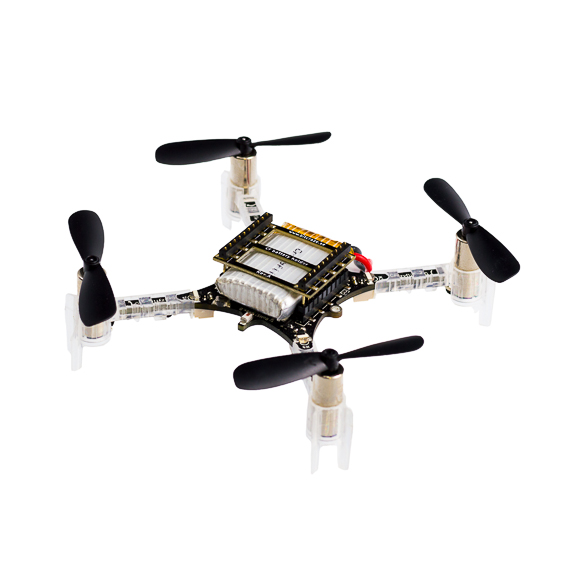
\includegraphics[scale=1]{crazyflie_new}}
	\end{picture}
\end{frame}

%%%%%%%%%%%%%%%%%%%%%%%%%%%%%%%%%%%%%%%%%%%%%%%%%%%%%%
%%%%%%%%%%%%%%%%%%%%%%%%%%%%%%%%%%%%%%%%%%%%%%%%%%%%%%
\section{\scshape Background}

%why necessary
%gapflyt
%flying indoors
%crazyflie size comparison
\begin{frame}{Background: UAV Flight}
	\vspace{-40pt}
	\begin{itemize}
		\item Autonomous navigation in \\constrained spaces 
		\begin{itemize}
			\item GapFlyt 
		\end{itemize}
		\item Small scale UAV control\\ + external sensors
		\begin{itemize}
			\item Crazyswarm
		\end{itemize}
		\item High level RNN controller
        
	\end{itemize}
	\begin{picture}(5.2, 3.4)
		\put(220,20){\includegraphics[scale=0.05]{gapflyt}}
	\end{picture}
	\begin{picture}(5.2, 3.4)
		\put(80,-60){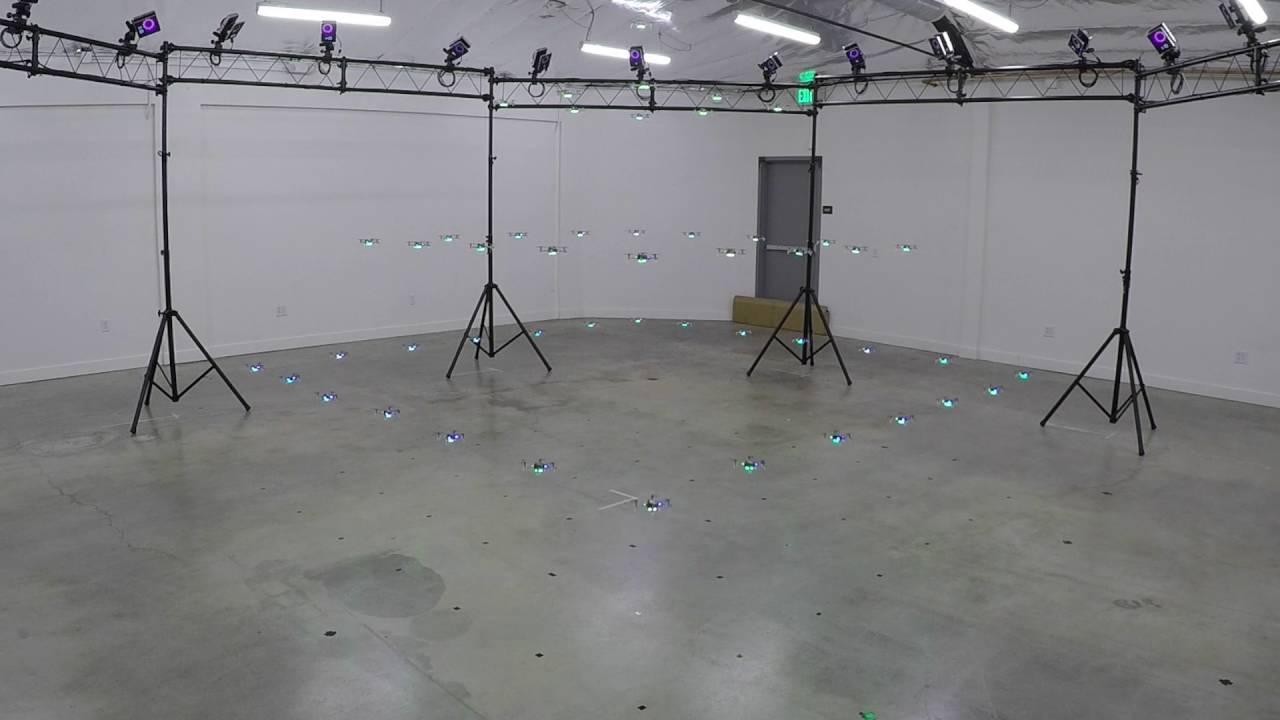
\includegraphics[scale=0.1]{crazyswarm}}
	\end{picture}
	\tiny{Source: \\\cite{gapflyt}\\ \cite{crazyswarm1}}
\end{frame}
\begin{frame}{Background: Door Detection}
	\begin{itemize}
		\item Networks: segment/bounding box
		\begin{itemize}
            \item U-Net
            \item MobileNet (V2)
            \item YOLO (Tiny)
		\end{itemize}
		\item Non-learning methods
		\begin{itemize}
            \item Corner, line, edge detection
            \item Fuzzy logic
		\end{itemize}
		\item Knowledge of full door- overkill for navigation?
	\end{itemize}
    \tiny{Source: \cite{parallelogram}, \cite{Unet}, \cite{howard2017mobilenets}, \cite{Fuzzy}, \cite{yolov3} }
\end{frame}


%%%%%%%%%%%%%%%%%%%%%%%%%%%%%%%%%%%%%%%%%%%%%%%%%%%%%%
%%%%%%%%%%%%%%%%%%%%%%%%%%%%%%%%%%%%%%%%%%%%%%%%%%%%%%
\section{\scshape Methodology}



\begin{frame}{Project Overview}
	\vspace{-10pt}
	\begin{itemize}
		\item Initial setup
		\begin{itemize}
			\item Motion capture
		\end{itemize}
		\item Door detection
		\item Independent Flight
	\end{itemize}
\end{frame}


\begin{frame}{Initial Setup}
    \vspace{-60pt}
    \begin{itemize}
        \item Payload redesign \& test flights
        \item Ground truth algorithm simulated \& VICON implementations
    \end{itemize}
    \href{run:../../images/VICON_flight.mp4}{Waypoint Navigation}
	\begin{picture}(3.2, 3.4)
		\put(70,60){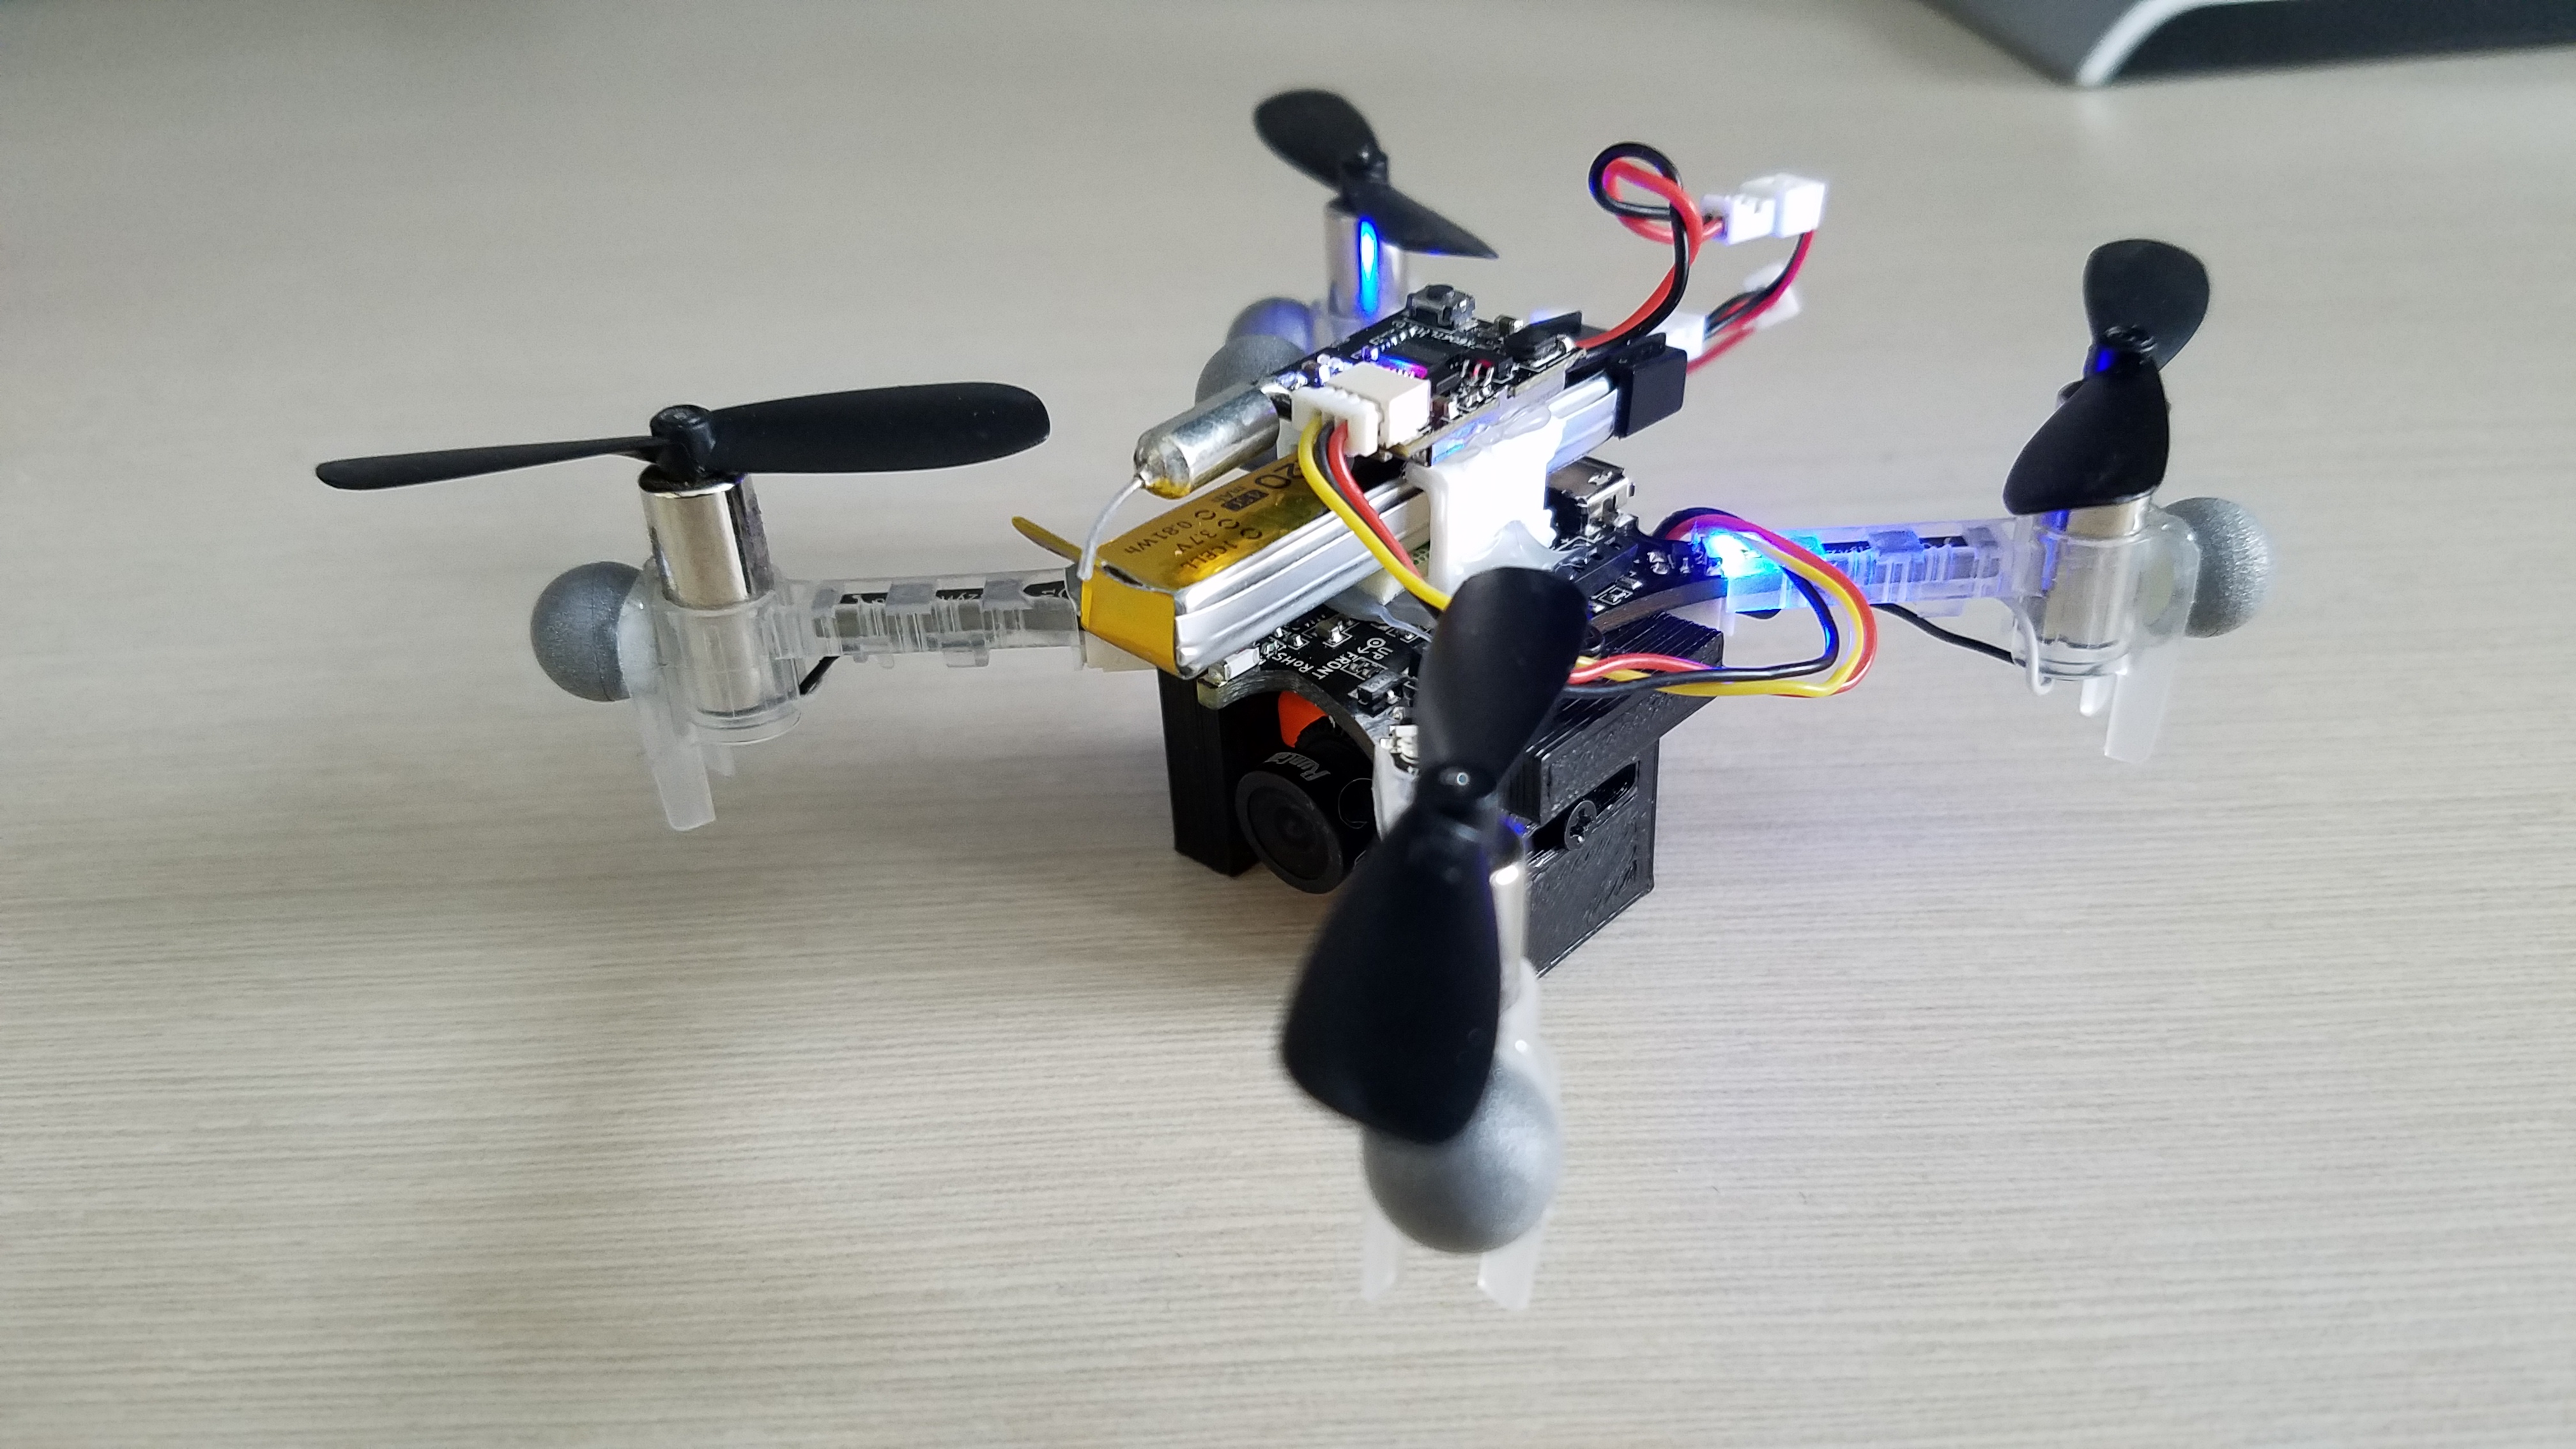
\includegraphics[scale=0.035]{payload1}}
	\end{picture}
	\begin{picture}(5.2, 3.4)
		\put(50,-100){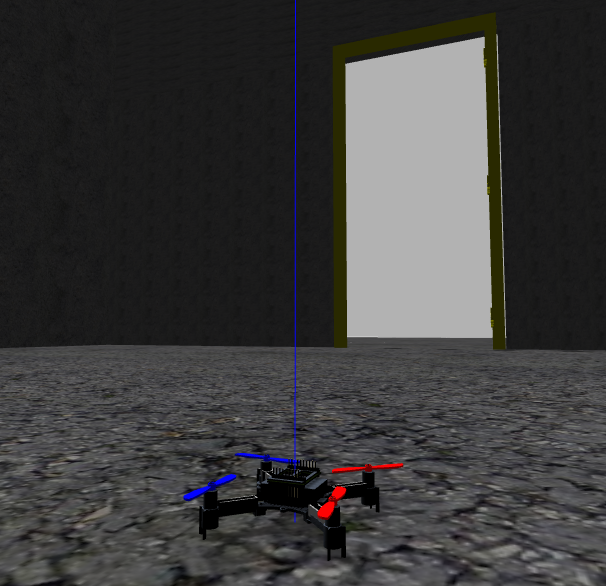
\includegraphics[scale=0.23]{gazebo}}
	\end{picture}
\end{frame}

\subsection{Door Detection}

\begin{frame}{Door Detection - Hough Transform}
    \bigskip
	\begin{picture}(5.2, 3.4)
		\put(-10,-70){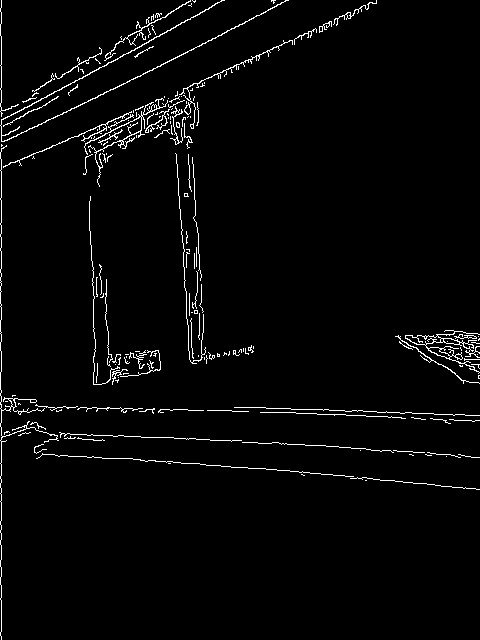
\includegraphics[scale=0.2]{canny}} %canny
	\end{picture}
	\begin{picture}(5.2, 3.4)
        \put(90,-70){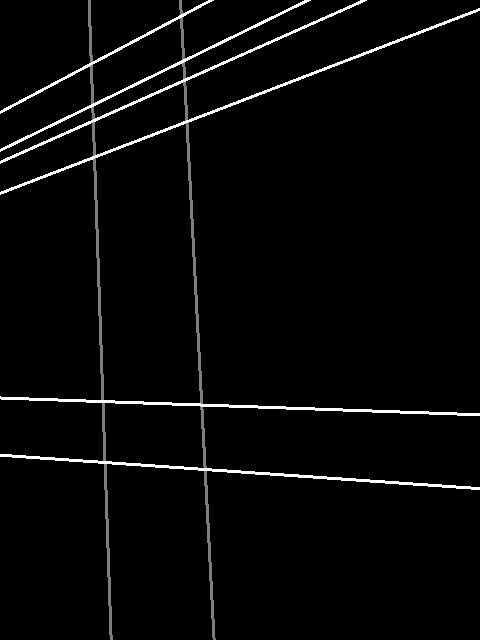
\includegraphics[scale=0.2]{lines}} %hough lines
	\end{picture}
	\begin{picture}(5.2, 3.4)
		\put(190,-70){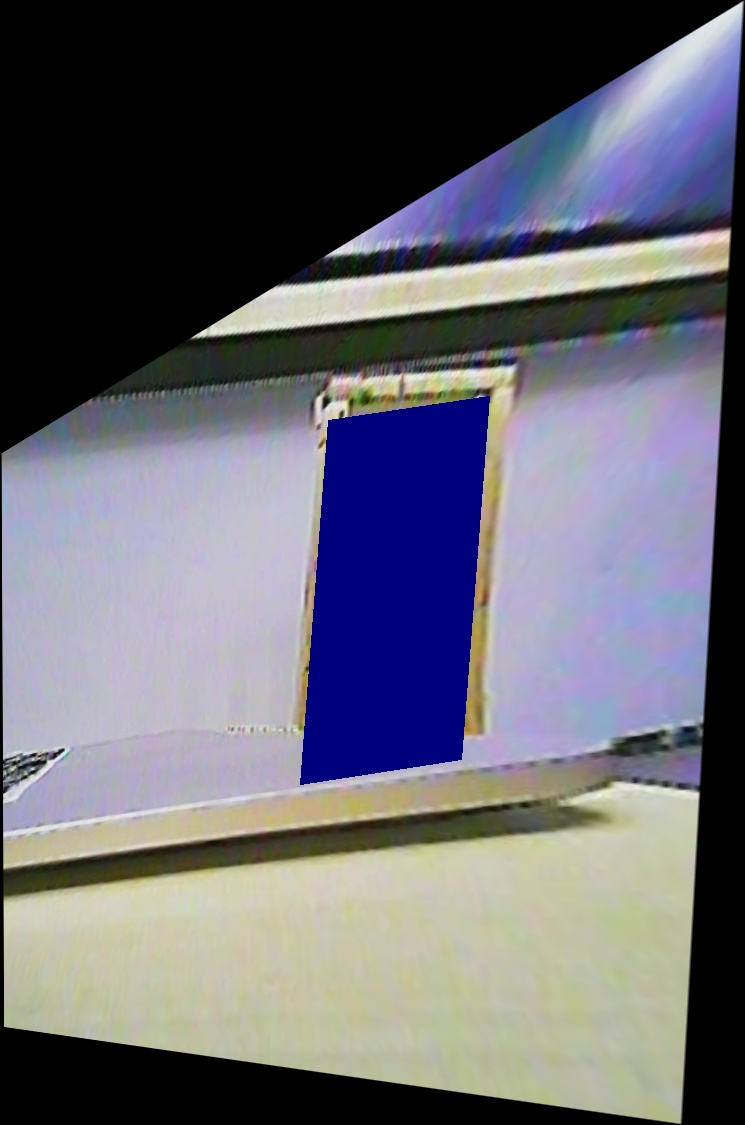
\includegraphics[scale=0.1129]{rectified_image}} %rectified
	\end{picture}
    \vfill
    \vspace{20pt}
%    \href{run:../../images/door_detection_hough_w_tracker.avi}{Initialization/Tracking}
\end{frame}


\begin{frame}{Door Detection - Convolutional Neural Net}
	\begin{picture}(5.2, 3.4)
        \centering
        \hspace{60pt}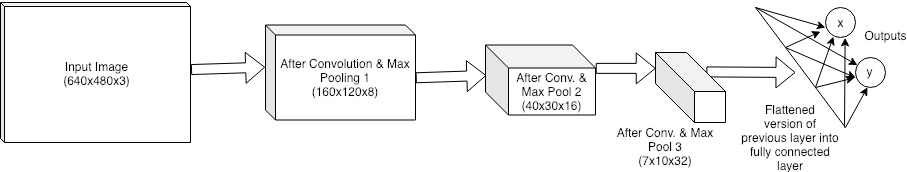
\includegraphics[scale=0.20]{arch}
	\end{picture}
	\begin{itemize}
        \item Small networks- ground station resources
        \item U-net, Tiny YOLO v3, MobileNet, own design
	\end{itemize}

    %    \href{run:../../images/door_detection_nn.avi}{Detection- Training Set}

	\begin{picture}(5.2, 3.4)
		\put(250,80){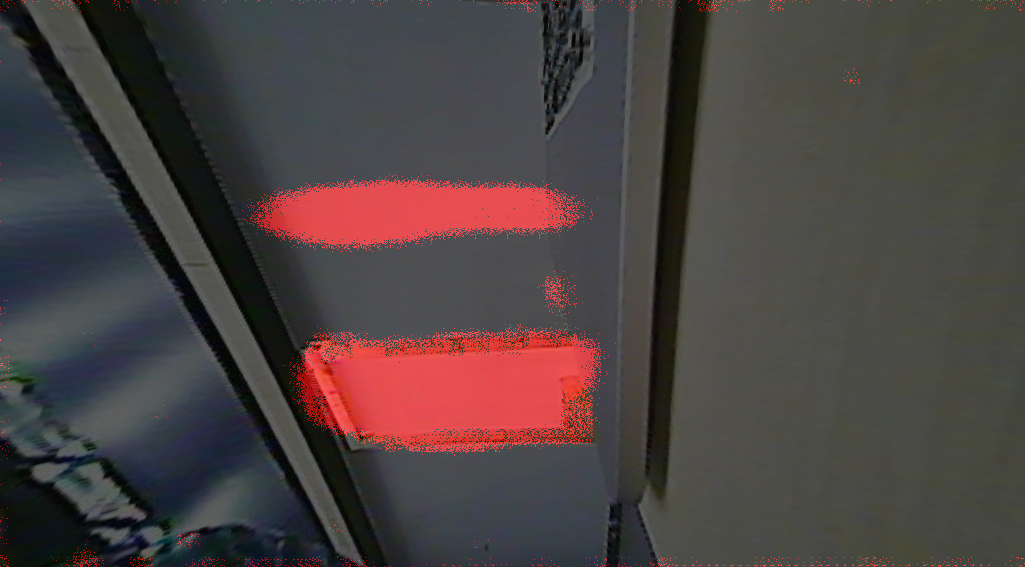
\includegraphics[scale=0.15,angle=270]{Unet_output}}
	\end{picture}

\end{frame}

\begin{frame}{Door Detection - YOLO}
	\begin{itemize}
        \item Small
        \item Fast
        \item Modified Loss Function
	\end{itemize}
    \begin{equation}
        \begin{aligned}
            \sum_{i = 0}^{48} \biggl( \lambda \mathlarger{\mathbbm{1}}_i^{\text{obj}}\bigl((x_i - \hat{x}_i)^2 + (y_i - \hat{y}_i)^2 + (\sqrt{w_i} - \sqrt{\hat{w}_i})^2 + \\
            (\sqrt{h_i} -\sqrt{\hat{h}_i})^2\bigr) + \sum_{c \in \text{classes}} (p_i(c) - \hat{p}_i(c))^2 \biggr)
        \end{aligned}
    \end{equation}
    \tiny\cite{yolov3}
\end{frame}



\subsection{Independent Flight}
\begin{frame}{Independent Flight - PD Control}
	\begin{itemize}
        \item $RollError = x_{ImageCenter}  - x_{DetectedDoorCenter}$
        \item $ThrustError = y_{ImageCenter}  - y_{DetectedDoorCenter}$
        \item $Command = K_{p}*Error + K_{d} * \frac{dError}{dt}$
	\end{itemize}

%    \href{run:../../images/ground_truth_sim.mp4}{Ground Truth}
\end{frame}

\begin{frame}{Independent Flight - Recurrent Neural Network}
	\begin{itemize}
		\item Hundreds of ground truth flights recorded
        \begin{itemize}
            \item Inputs: IMU, image, time
            \item Output: Roll/Pitch/Thrust/Yaw-rate
        \end{itemize}
        \item Image - convolutional section
        \item Inputs/Outputs normalized
        \item Gated Recurrent Units (GRU) - memory 
	\end{itemize}
	\begin{picture}(5.2, 3.4)
		\put(250,-20){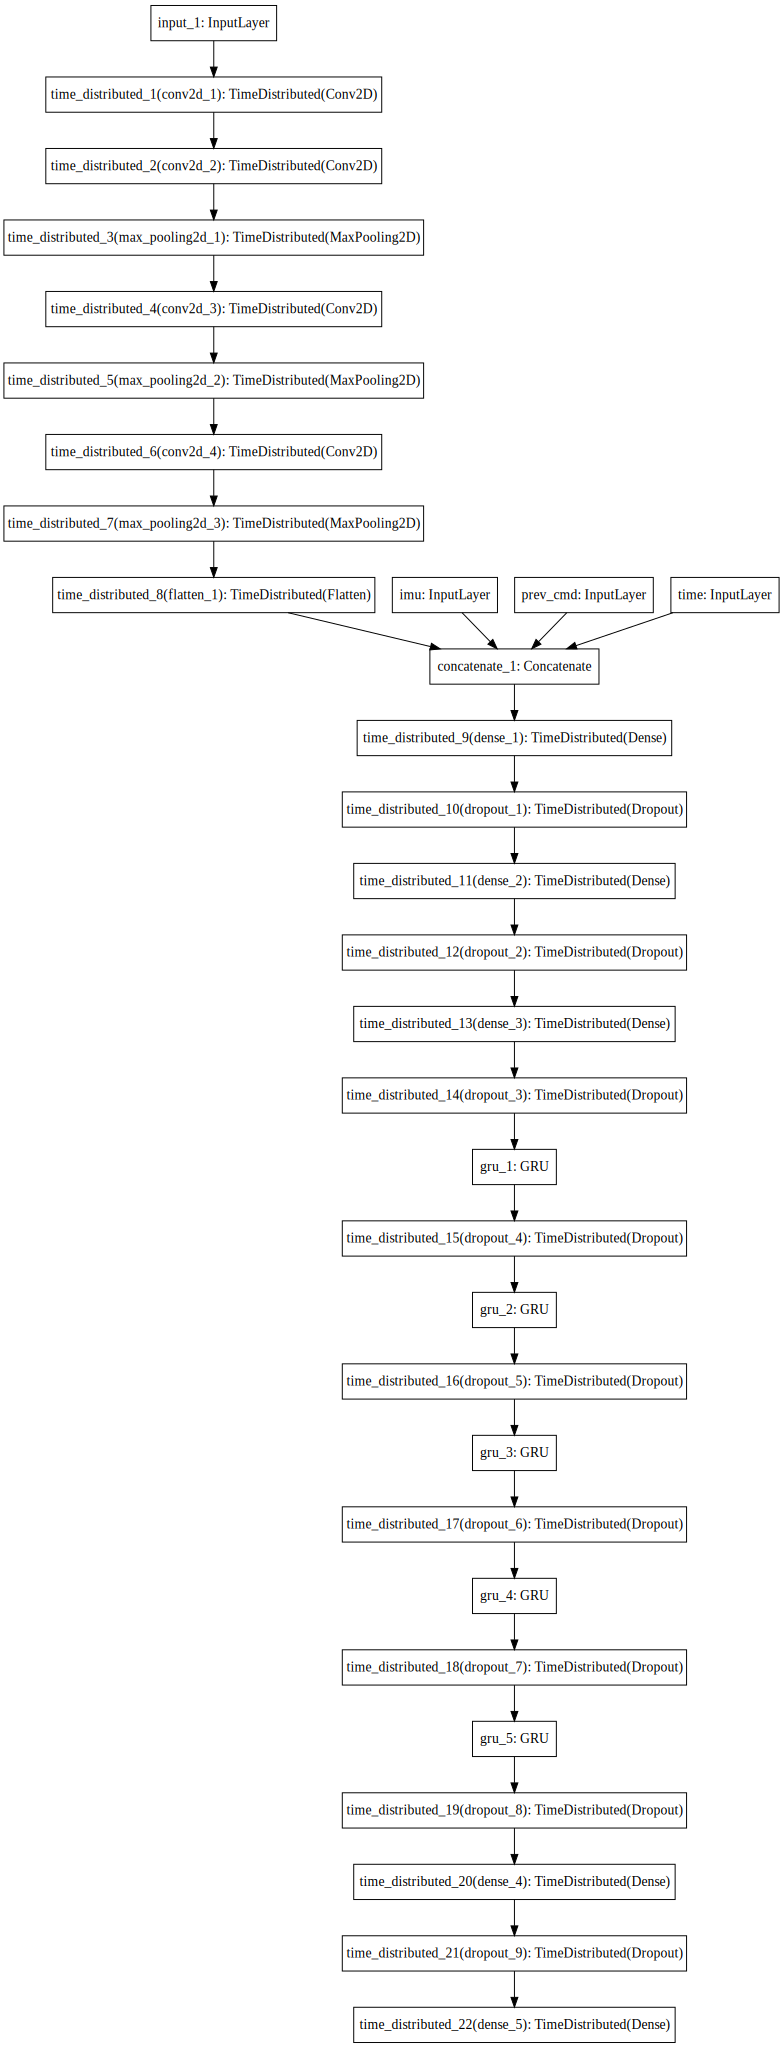
\includegraphics[scale=0.023]{model}}
	\end{picture}
    \tiny\cite{GRU}
\end{frame}


\section{Results}
\begin{frame}{Door Detection - Timing Comparison}

On fake door set:

\begin{table}[H]
\begin{tabular}{lll}
\begin{tabular}[c]{@{}l@{}}\end{tabular} & Hough Method   & CNN \\
Mean msec/image            & 1.11 & 0.89              \\
Std. dev. msec/image       & 1.99 & 0.024             \\
\end{tabular}
\end{table}

\hline
\vspace{10pt}
On real door set:

\begin{table}[H]
\begin{tabular}{lll}
\begin{tabular}[c]{@{}l@{}}\end{tabular} & Hough Method   & CNN \\
Mean msec/image            & 0.08 & 0.072              \\
Std. dev. msec/image       & 0.02 & 0.009             \\
\end{tabular}
\end{table}

\end{frame}

\begin{frame}{Door Detection - Accuracy Comparison}

	\begin{picture}(5.2, 3.4)
		\put(160,-100){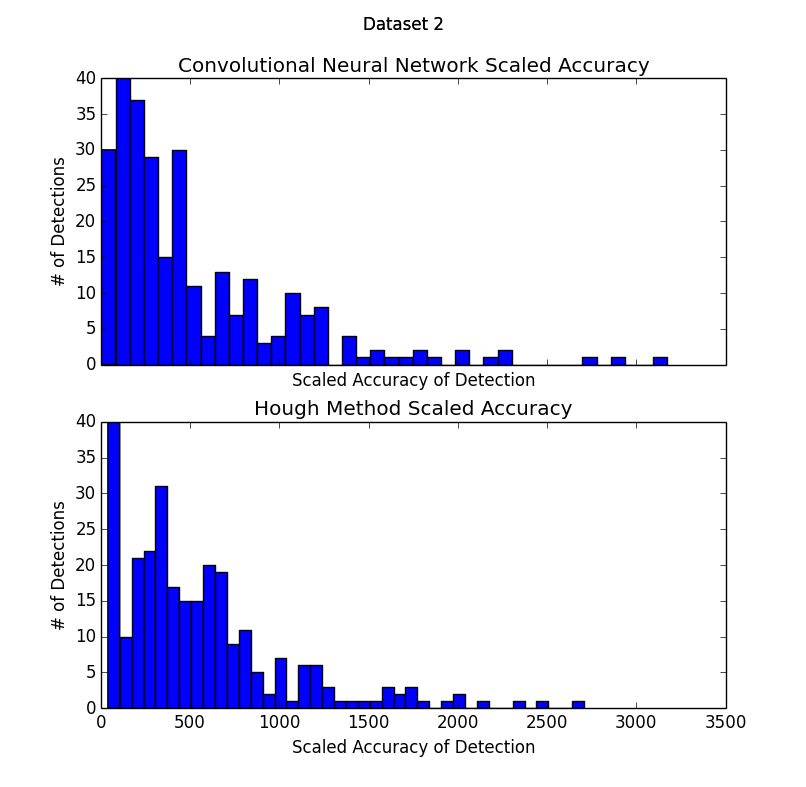
\includegraphics[scale=0.3]{AccuracyComparison2}}
	\end{picture}
	\begin{picture}(5.2, 3.4)
		\put(-40,-100){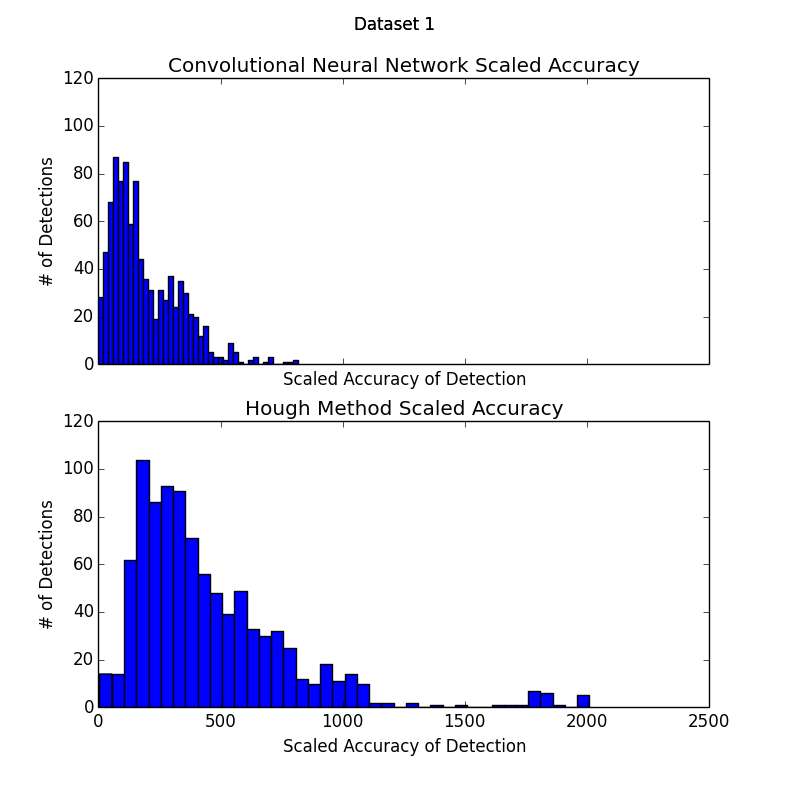
\includegraphics[scale=0.3]{AccuracyComparison1}}
	\end{picture}


\end{frame}

\begin{frame}{Independent Flight - Success Comparison}
	\begin{itemize}
		\item Zero location selected
        \begin{itemize}
            \item PD controller tuned from zero location
            \item Network trained on flights from zero location
        \end{itemize}
        \item 20 flights from zero location, 20 from arbitrary location
        
	\end{itemize}

%\begin{table}[]
%\resizebox{\columnwidth}{!} {
%\begin{tabular}{lll}
%\hline
%                                     & PD Control   & RNN Control            \\ \hline
%Stable Flight                        & Yes          & Yes                    \\
%Success rate from zero location      & 65\% (13/20) & Loops w/o finding door \\
%Success rate from arbitrary location & 25\% (5/20)  & Loops w/o finding door
%\end{tabular}
%}
%\end{table}
\begin{table}[]
    \resizebox{\columnwidth}{!}{
\begin{tabular}{l|l|l|}
\cline{2-3}
                                                           & PD Control   & RNN Control            \\ \hline
\multicolumn{1}{|l|}{Stable Flight}                        & Yes          & Yes                    \\ \hline
\multicolumn{1}{|l|}{Success rate from zero location}      & 65\% (13/20) & Loops w/o finding door \\ \hline
\multicolumn{1}{|l|}{Success rate from arbitrary location} & 25\% (5/20)  & Loops w/o finding door \\ \hline
\end{tabular}
}
\end{table}



\end{frame}

\begin{frame}{Independent Flight - Successful Flight}

	\begin{picture}(5.2, 3.4)
		\put(0,-100){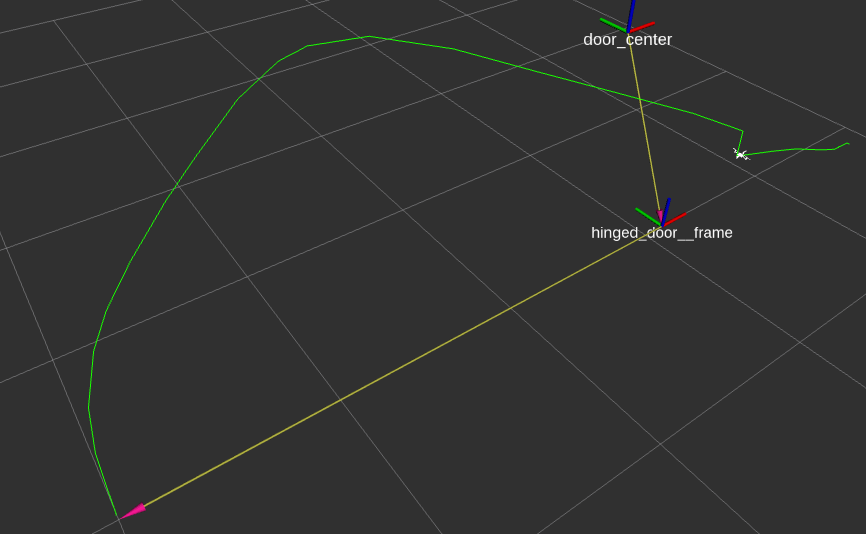
\includegraphics[scale=0.35]{rviz_angle}}
	\end{picture}

\end{frame}

\section{\scshape Conclusion}


\begin{frame}{Conclusion}
%	\vspace{-60pt}
	\begin{itemize}
		\item Explored intersection of small size, auto navigation
		\item Compare methods for door detection
            \begin{itemize}
                \item CNN more accurate, faster
            \end{itemize}
		\item Compare methods for independent flight
            \begin{itemize}
                \item PD controller capable of navigating UAV through door based on door detection
            \end{itemize}
	\end{itemize}
\end{frame}

\begin{frame}
	Questions
\end{frame}

\begin{frame}{References}
    \vspace{-20pt}
	\tiny{\bibliography{../../references}}
\end{frame}

\begin{frame}{Simulation}
	\begin{itemize}
		\item Gazebo Simulator 
        \item Input/Output same form as real Crazyflie (SITL)
		\item Noisy, low resolution camera
		\item Noise IMU
		\item Delay to mimic data down-link
	\end{itemize}
\end{frame}

\begin{frame}{Motion Capture}
	\begin{itemize}
		\item VICON
		\item Set of cameras
		\item Track balls on desired object
		\item Provide orientation/position but only w/i tracked space
		\item Safety net: bad UAV orientation/path = shut down
	\end{itemize}
	\begin{picture}(5.2, 3.4)
		\put(120,90){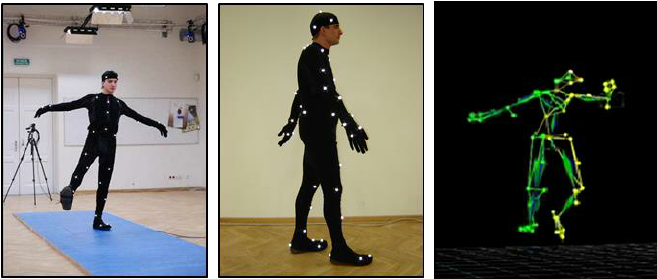
\includegraphics[scale=0.3]{mocap}}
		\tiny{Source: \cite{mocap}}
	\end{picture}

\end{frame}

\begin{frame}{Hough Transform}
	\begin{itemize}
		\item Edge detector
		\item Parametrize line:
		\item $r = x*cos(\theta) + y*sin(\theta)$
		\item For each edge point: determine all $r$, $\theta$ solving above, increment table
		\item Maximums of table give lines majority of points agree on 
	\end{itemize}
	\begin{tikzpicture}[scale=1]
	    % Draw axes
	    \draw [<->,thick] (0,2) node (yaxis) [above] {$\theta$}
		|- (3,0) node (xaxis) [right] {$r$};
	\end{tikzpicture}
	\vspace{10pt}

\end{frame}



\end{document}
